\newsavebox{\mazetablebox}
\sbox{\mazetablebox}{%
  \begin{minipage}[b]{0.63\textwidth}
    \centering
    \scriptsize

    \label{tab:sim_maze_results}

    \begin{tabular}{lccc}
        \toprule
Metric & \textbf{\textcolor[HTML]{66C2A5}{McVAMP}} & \textbf{\textcolor[HTML]{FC8D62}{ReVAMP w/o EECC}} & \textbf{\textcolor[HTML]{8DA0CB}{ReVAMP}} \\
\midrule
Success (\%) & 88.5 & 89.0 & \textbf{89.5} \\
Iterations & 9442 (14644 $\pm$ 17872) & \textbf{5183 (11503 $\pm$ 16680)} & 5283 (11365 $\pm$ 17355) \\
Resolve (ms) & -- & 0.01 (0.01 $\pm$ 0.02) & \textbf{0.01 (0.01 $\pm$ 0.01)} \\
Planning (ms) & 46.19 (71.78 $\pm$ 92.21) & 5.52 (9.91 $\pm$ 11.91) & \textbf{4.38 (7.33 $\pm$ 8.72)} \\
Shortcut (ms) & 12.14 (16.75 $\pm$ 13.87) & 0.60 (0.69 $\pm$ 0.43) & \textbf{0.42 (0.48 $\pm$ 0.30)} \\
Total (ms) & 59.80 (88.53 $\pm$ 97.87) & 6.14 (10.60 $\pm$ 12.07) & \textbf{4.76 (7.81 $\pm$ 8.83)} \\
Failure (ms) & 473.22 (463.89 $\pm$ 68.89) & 75.01 (78.45 $\pm$ 19.56) & \textbf{57.31 (60.15 $\pm$ 18.17)} \\
Config dist. (rad) & \textbf{10.81 (10.75 $\pm$ 2.58)} & 11.57 (12.06 $\pm$ 4.14) & 11.49 (11.70 $\pm$ 3.74) \\
EEF dist. & 7.21 (7.30 $\pm$ 2.21) & 6.43 (5.71 $\pm$ 2.16) & \textbf{6.37 (5.47 $\pm$ 2.06)} \\
\bottomrule

\end{tabular}
    \captionof{table}{Maze Experiment Results: Median (Mean $\pm$ Std.) Planning Times and Path Lengths}
  \end{minipage}%
}

\begin{figure*}[!t]
\centering
% \begin{tabular} sets its own box's reference point (baseline) near its
% vertical center, not its visual bottom -- a well-known LaTeX quirk -- so a
% plain minipage[b] wrapping a tabular does NOT align to the bottom rule.
% \raisebox{\dp}{...} (a plain lift, NOT the [height][depth] override form,
% which only overrides reported metrics without moving the ink) shifts
% \mazetablebox up by its own depth, which moves its reference point to
% coincide with its true visual bottom (the bottom rule). The image+caption
% column is ordinary text, whose minipage[b] reference point is already its
% own bottom (the caption's last line), so it needs no such correction.
% With both reference points at their visual bottoms, plain side-by-side
% placement aligns them -- no manual offset to re-tune.
\raisebox{\dp\mazetablebox}{\usebox{\mazetablebox}}%
\hfill
\begin{minipage}[b]{0.36\textwidth}
    \centering
    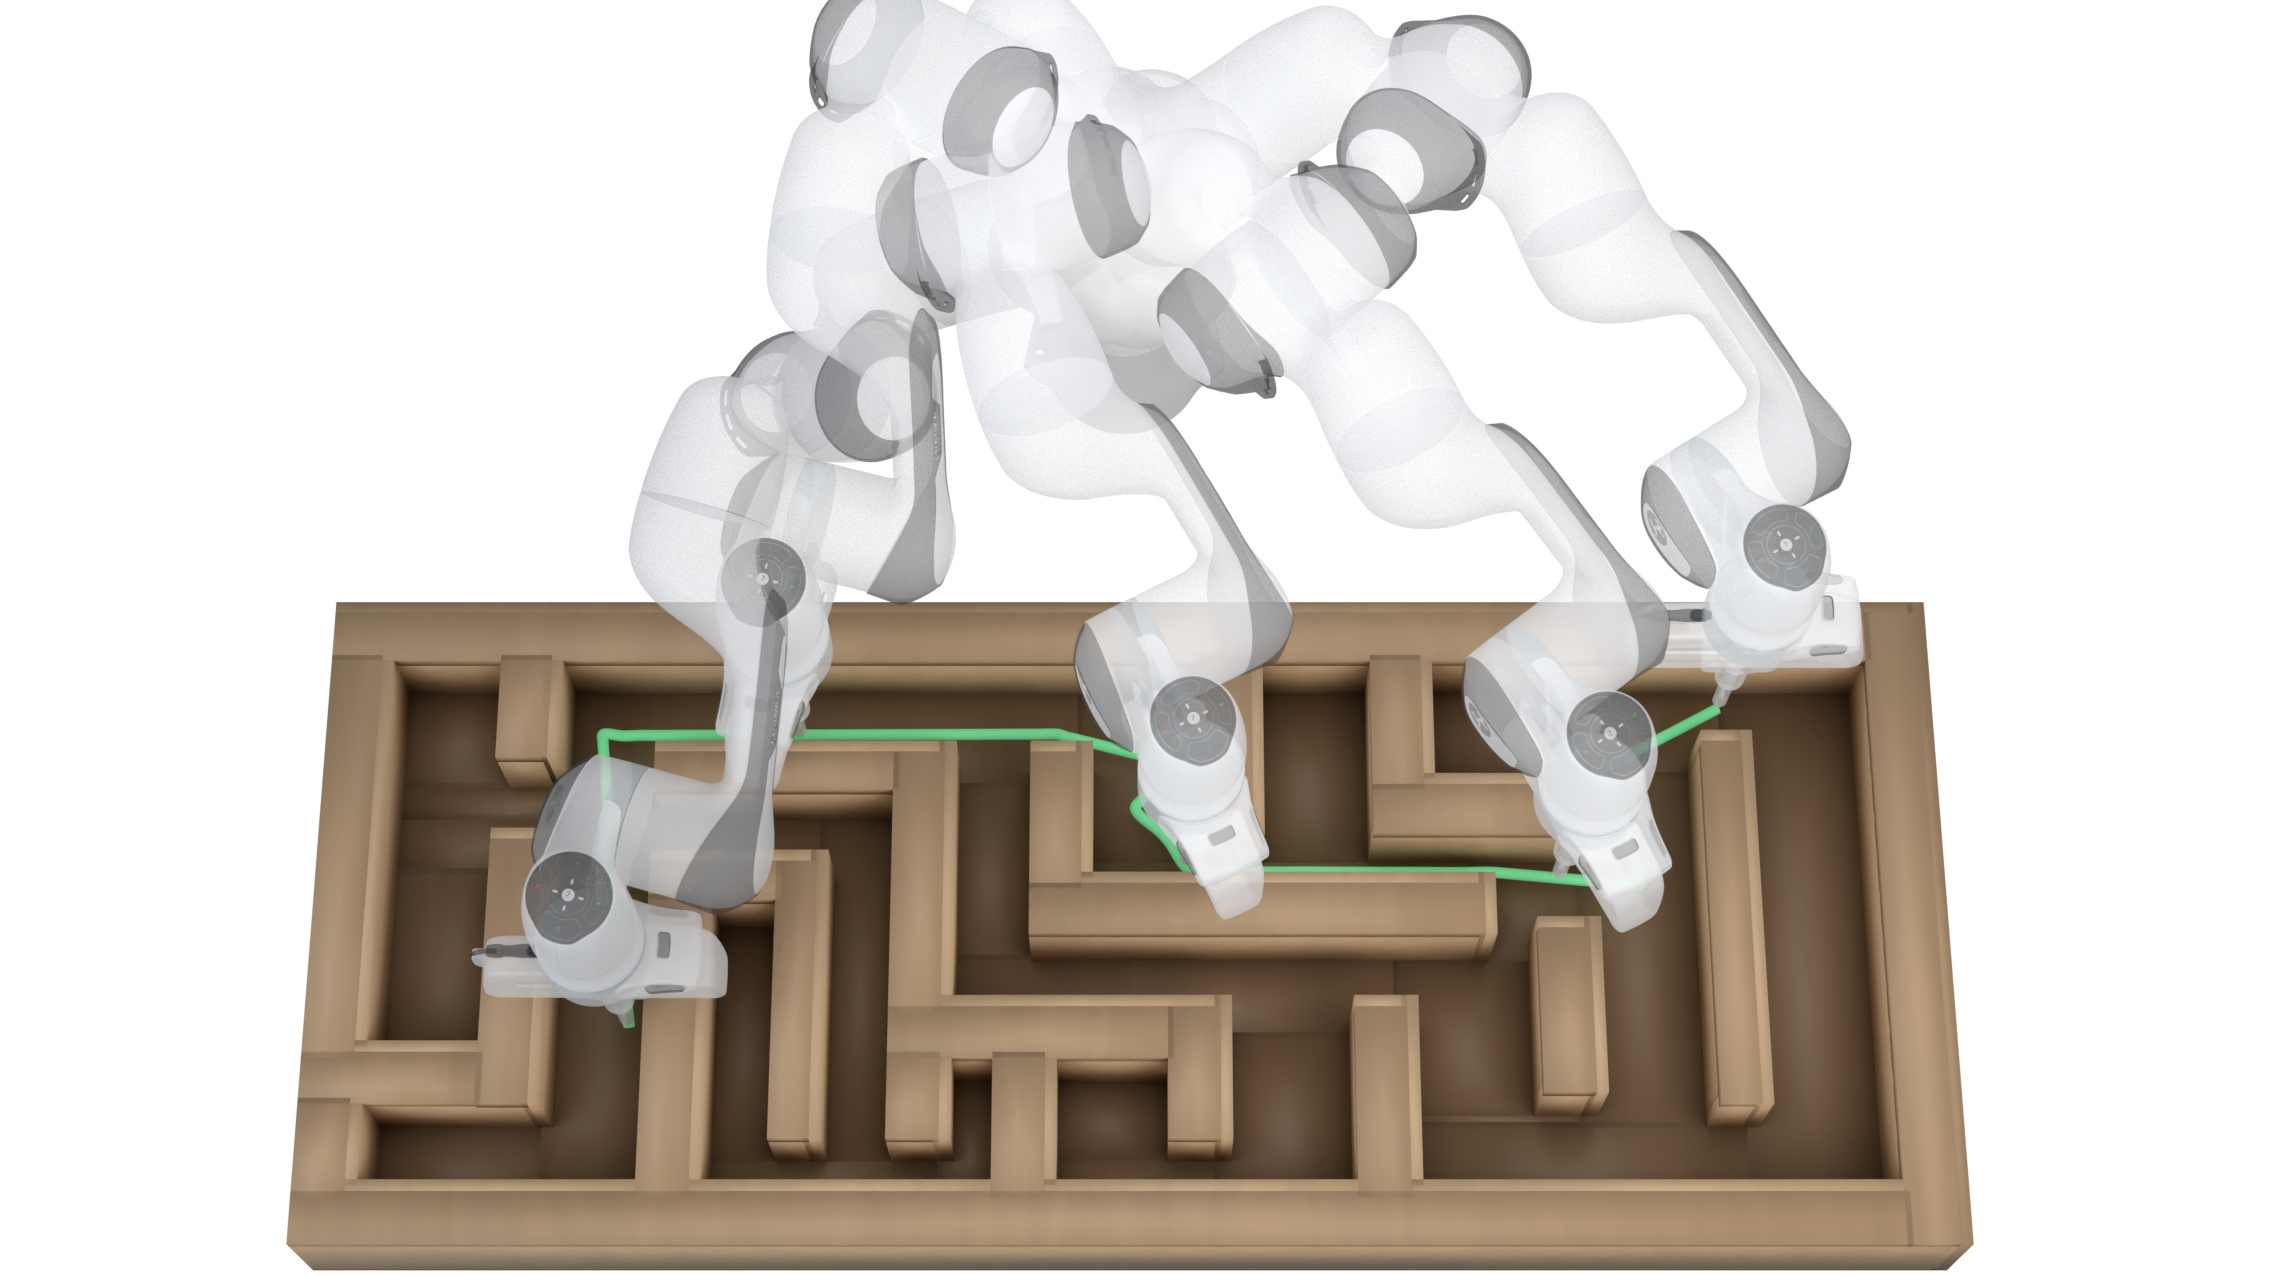
\includegraphics[width=\linewidth]{images/hero_ghosts.jpg}\par
    \captionof{figure}{Example of a solved trajectory in the maze.}
    \label{fig:maze_hero}
\end{minipage}
\end{figure*}
